\documentclass{standalone}
\usepackage{tikz}
\usepackage{gensymb}

\tikzset{every picture/.style={line width=0.75pt}} %set default line width to 0.75pt


\begin{document}

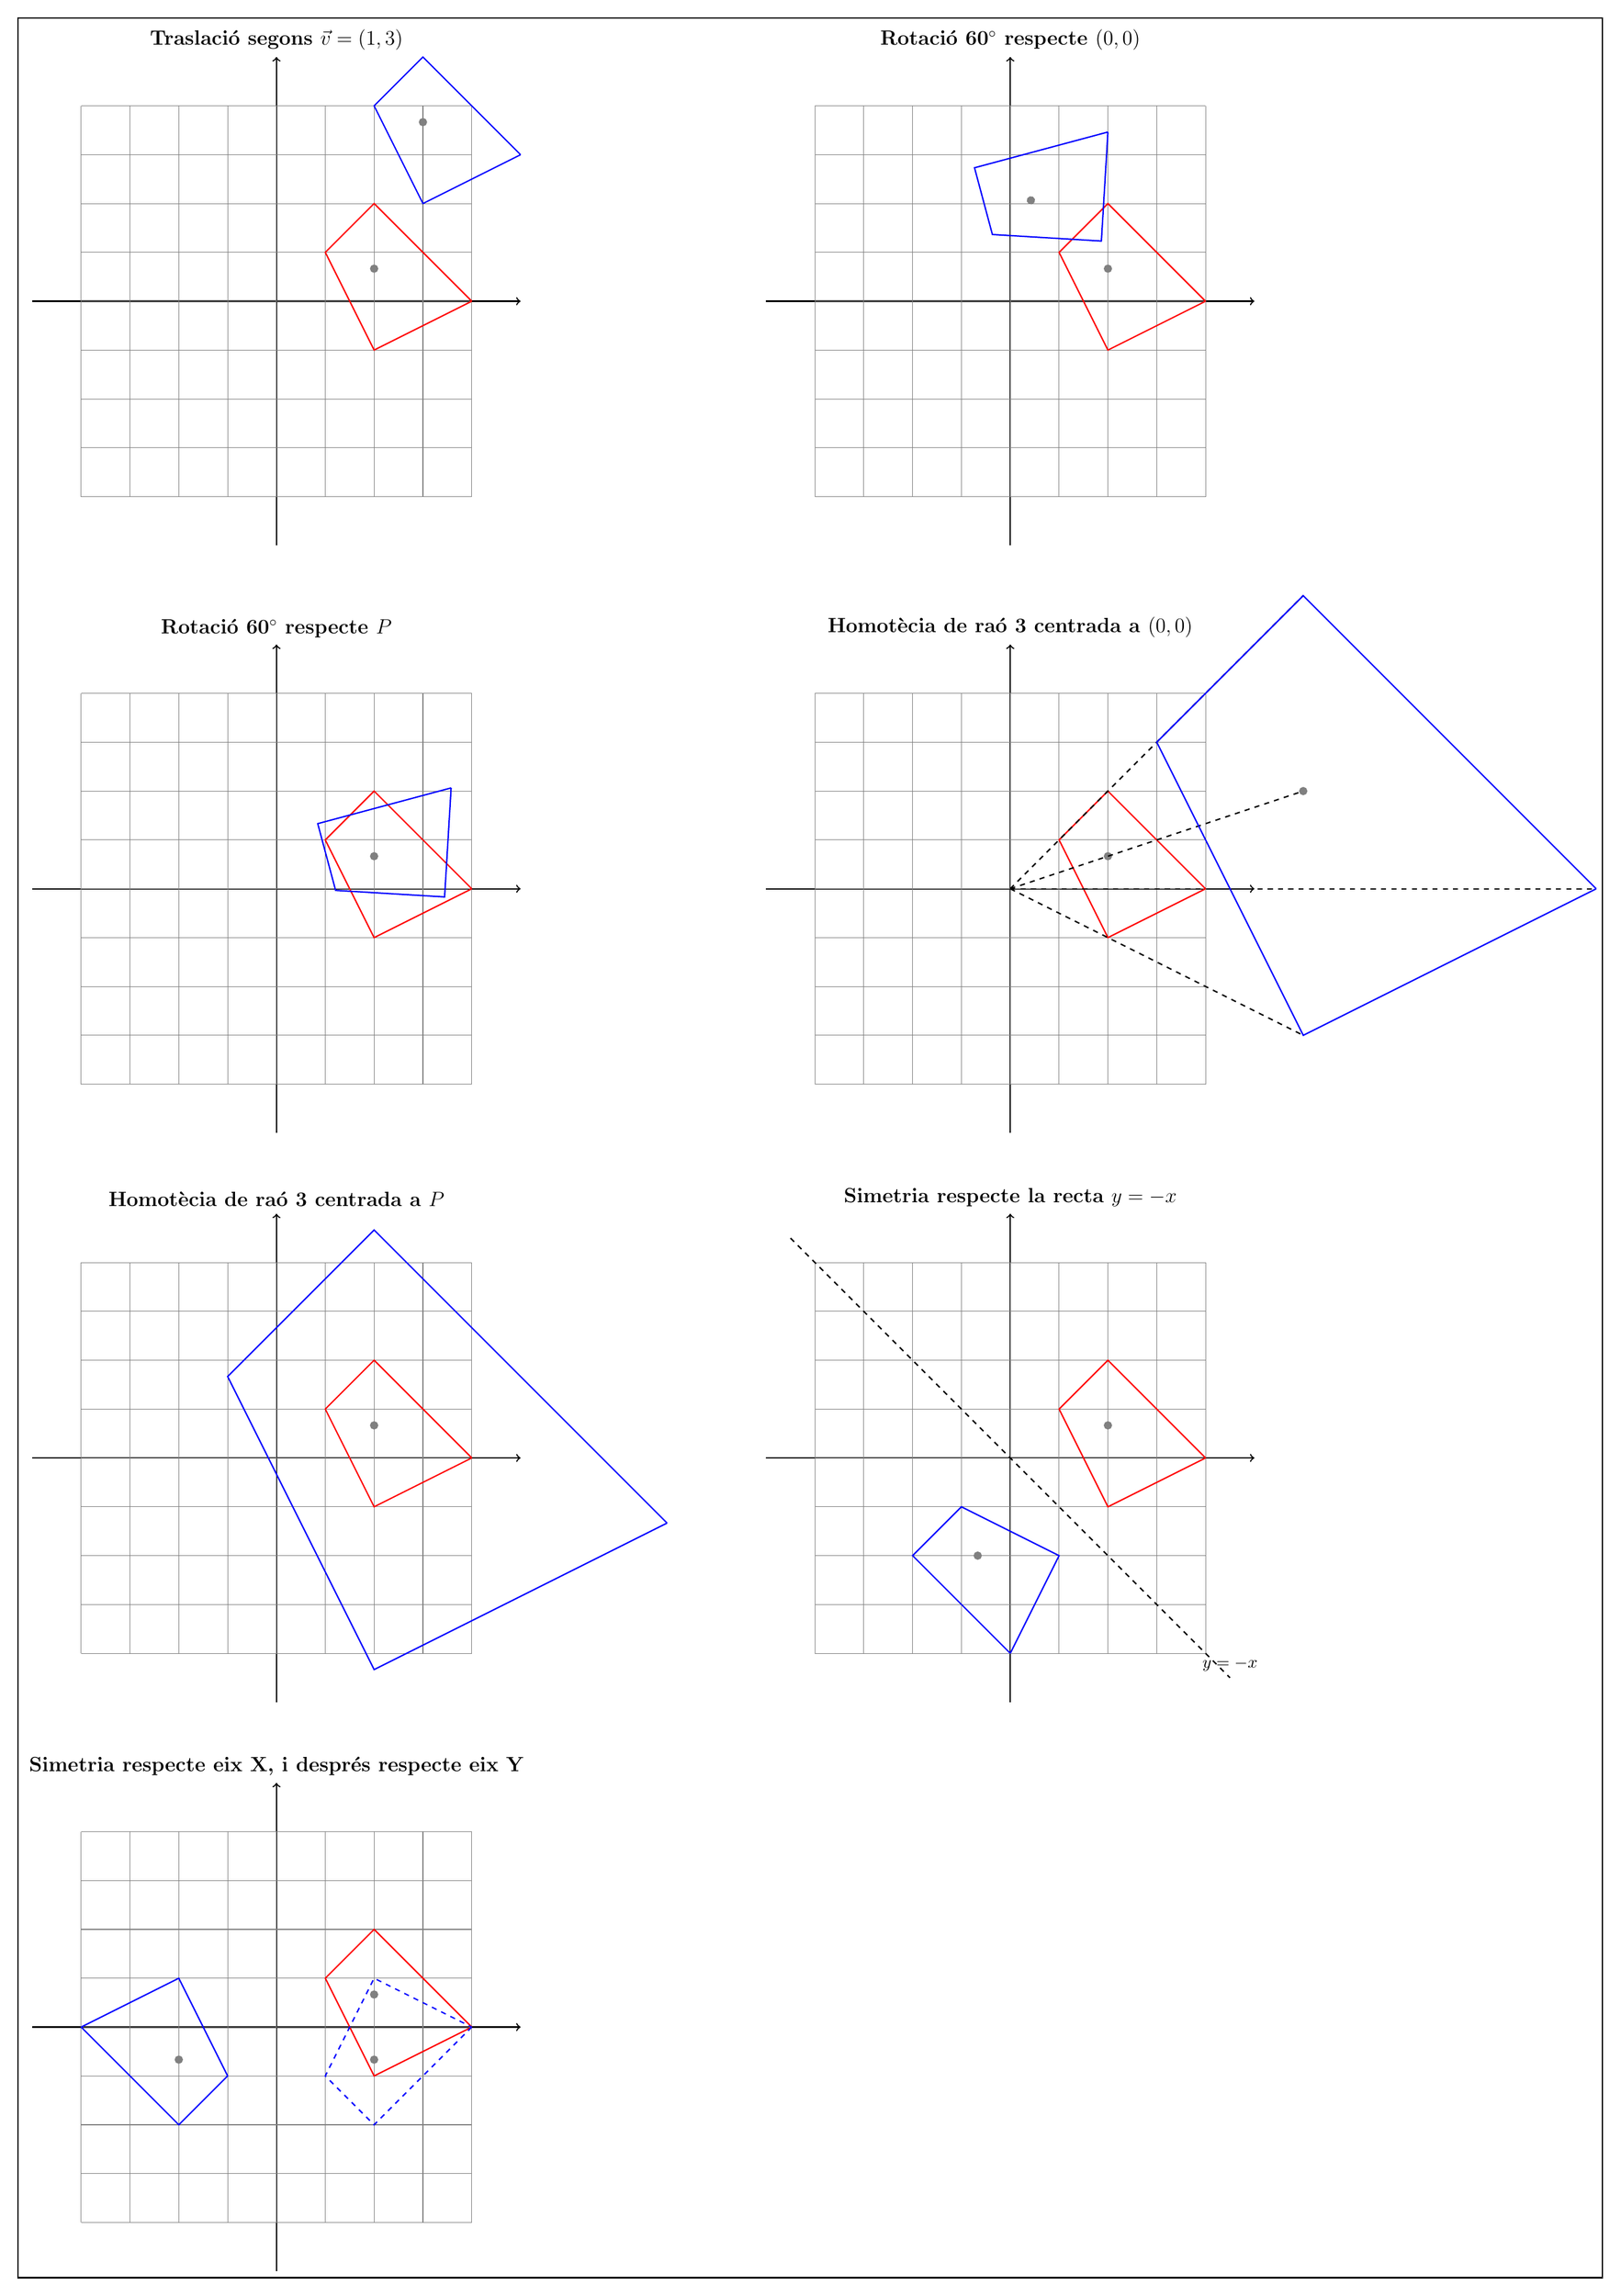
\begin{tikzpicture}[scale = 0.25]

\matrix[
      draw,
      thick,
      column sep=2cm,
      row sep=1cm
]{
%%%%%%%%%%%%%%%%%%%%%%%%%%%%%%%%%%%%%%%%%%%%%%%%%%%
%%%%%%%%%%%%%%%%%%%%%%%%%%%%%%%%%%%%%%%%%%%%%%%%%%%
% traslació segons vector (1,3)
\draw [->](-5,0) -- (5,0); %x-axis
\draw [->](0,-5) -- (0,5); %y-axis
\draw [step=1.0,gray,thin] (-4,-4) grid (4,4);
\node[above,font=\large\bfseries] at (current bounding box.north) {Traslació segons $\vec{v}=(1,3)$};
%\draw[red] (4,0) -- (2,2) -- (1,1) -- (2,-1) -- (4,0);
\draw[red] (4,0) -- (2,2) -- (1,1) -- (2,-1) -- (4,0);
\filldraw [gray] (2,2/3) circle (2pt);
\begin{scope}[shift={(1,3)}]
  \draw[blue] (4,0) -- (2,2) -- (1,1) -- (2,-1) -- (4,0);
  \filldraw [gray] (2,2/3) circle (2pt);
\end{scope}
&
% rotació 60 graus respecte origen
\draw [->](-5,0) -- (5,0); %x-axis
\draw [->](0,-5) -- (0,5); %y-axis
\draw [step=1.0,gray,thin] (-4,-4) grid (4,4);
\node[above,font=\large\bfseries] at (current bounding box.north) {Rotació 60$\degree$ respecte $(0,0)$};
\draw[red] (4,0) -- (2,2) -- (1,1) -- (2,-1) -- (4,0);
\filldraw [gray] (2,2/3) circle (2pt);
\begin{scope}[rotate=60]
  \draw[blue] (4,0) -- (2,2) -- (1,1) -- (2,-1) -- (4,0);
  \filldraw [gray] (2,2/3) circle (2pt);
\end{scope}

\\
%%%%%%%%%%%%%%%%%%%%%%%%%%%%%%%%%%%%%%%%%%%%%%%%%%%
%%%%%%%%%%%%%%%%%%%%%%%%%%%%%%%%%%%%%%%%%%%%%%%%%%%
% rotació 60 graus respecte el punt D
\draw [->](-5,0) -- (5,0); %x-axis
\draw [->](0,-5) -- (0,5); %y-axis
\draw [step=1.0,gray,thin] (-4,-4) grid (4,4);
\node[above,font=\large\bfseries] at (current bounding box.north) {Rotació 60$\degree$ respecte $P$};
\draw[red] (4,0) -- (2,2) -- (1,1) -- (2,-1) -- (4,0);
\filldraw [gray] (2,2/3) circle (2pt);
\draw[blue,rotate around={60:(2,2/3)}] (4,0) -- (2,2) -- (1,1) -- (2,-1) -- (4,0);
&
% homotècia de raó 3 centrada a l'origen
\draw [->](-5,0) -- (5,0); %x-axis
\draw [->](0,-5) -- (0,5); %y-axis
\draw [step=1.0,gray,thin] (-4,-4) grid (4,4);
\node[above,font=\large\bfseries] at (current bounding box.north) {Homotècia de raó 3 centrada a $(0,0)$};
\draw[red] (4,0) -- (2,2) -- (1,1) -- (2,-1) -- (4,0);
\filldraw [gray] (2,2/3) circle (2pt);
\filldraw [gray] (6,2) circle (2pt);
\draw[black,dashed] (0,0) -- (6,6);
\draw[black,dashed] (0,0) -- (6,2);
\draw[black,dashed] (0,0) -- (12,0);
\draw[black,dashed] (0,0) -- (6,-3);
\draw[blue,scale=3] (4,0) -- (2,2) -- (1,1) -- (2,-1) -- (4,0);
\\
%%%%%%%%%%%%%%%%%%%%%%%%%%%%%%%%%%%%%%%%%%%%%%%%%%%
%%%%%%%%%%%%%%%%%%%%%%%%%%%%%%%%%%%%%%%%%%%%%%%%%%%
% homotècia de raó 3 centrada al punt D
\draw [->](-5,0) -- (5,0); %x-axis
\draw [->](0,-5) -- (0,5); %y-axis
\draw [step=1.0,gray,thin] (-4,-4) grid (4,4);
\node[above,font=\large\bfseries] at (current bounding box.north) {Homotècia de raó 3 centrada a $P$};
\draw[red] (4,0) -- (2,2) -- (1,1) -- (2,-1) -- (4,0);
\filldraw [gray] (2,2/3) circle (2pt);
\draw[blue,scale around={3:(2,2/3)}] (4,0) -- (2,2) -- (1,1) -- (2,-1) -- (4,0);
&
% simetria respecte la recta y=-x
\draw [->](-5,0) -- (5,0); %x-axis
\draw [->](0,-5) -- (0,5); %y-axis
\draw [step=1.0,gray,thin] (-4,-4) grid (4,4);
\node[above,font=\large\bfseries] at (current bounding box.north) {Simetria respecte la recta $y=-x$};
\draw[red] (4,0) -- (2,2) -- (1,1) -- (2,-1) -- (4,0);
\filldraw [gray] (2,2/3) circle (2pt);
\begin{scope}[cm={0,-1,-1,0,(0,0)}]
  \draw[blue] (4,0) -- (2,2) -- (1,1) -- (2,-1) -- (4,0);
  \filldraw [gray] (2,2/3) circle (2pt);
\end{scope}
\draw[black,dashed] (-4.5,4.5) -- (4.5,-4.5) node[above] {$y=-x$};
\\
%%%%%%%%%%%%%%%%%%%%%%%%%%%%%%%%%%%%%%%%%%%%%%%%%%%
%%%%%%%%%%%%%%%%%%%%%%%%%%%%%%%%%%%%%%%%%%%%%%%%%%%
% simetria respecte eix X, seguida per simetria respecte eix Y
\draw [->](-5,0) -- (5,0); %x-axis
\draw [->](0,-5) -- (0,5); %y-axis
\draw [step=1.0,gray,thin] (-4,-4) grid (4,4);
\node[above,font=\large\bfseries] at (current bounding box.north) {Simetria respecte eix X, i després respecte eix Y};
\draw[red] (4,0) -- (2,2) -- (1,1) -- (2,-1) -- (4,0);
\filldraw [gray] (2,2/3) circle (2pt);
\begin{scope}[cm={1,0,0,-1,(0,0)}]
  \draw[blue,dashed,] (4,0) -- (2,2) -- (1,1) -- (2,-1) -- (4,0);
  \filldraw [gray] (2,2/3) circle (2pt);
\end{scope}
\begin{scope}[cm={-1,0,0,-1,(0,0)}]
  \draw[blue] (4,0) -- (2,2) -- (1,1) -- (2,-1) -- (4,0);
  \filldraw [gray] (2,2/3) circle (2pt);
\end{scope}

&
\\
};

%
% \begin{scope}[rotate=60]
% \end{scope}
%
% \begin{scope}[rotate around={60:(2,2/3)}]
% \draw[cyan] (4,0) -- (2,2) -- (1,1) -- (2,-1) -- (4,0) node[below left] {$c$};
% \end{scope}
%
% \begin{scope}[scale=3]
% \draw[yellow] (4,0) -- (2,2) -- (1,1) -- (2,-1) -- (4,0) node[below left] {$d$};
% \end{scope}
%
% \begin{scope}[scale around={3:(2,2/3)}]
% \draw[orange] (4,0) -- (2,2) -- (1,1) -- (2,-1) -- (4,0) node[below left] {$d$};
% \end{scope}

%
% \begin{scope}[cm={0,-1,-1,0,(0,0)}]
% \draw[pink] (4,0) -- (2,2) -- (1,1) -- (2,-1) -- (4,0) node[below left] {$e$};
% \end{scope}

% \begin{scope}[cm={-1,0,0,-1,(0,0)}]
% \draw[black] (4,0) -- (2,2) -- (1,1) -- (2,-1) -- (4,0) node[below left] {$e$};
% \end{scope}


\end{tikzpicture}

\end{document}
